\documentclass[a4paper, 11pt]{article}
\usepackage[ngerman]{babel}
%ä und so
\usepackage[utf8]{inputenc}
\usepackage[T1]{fontenc}
\usepackage{amsmath}
\usepackage{amsthm}
\usepackage{amsbsy}

\usepackage{mathrsfs}
\usepackage{amssymb}
\usepackage{amstext}
\usepackage{amsfonts}
\usepackage{float}
\usepackage{graphicx}
\usepackage{esdiff}
\usepackage{hyperref}

\begin{document}
\title{E-Lehre}
\author{Gruppe B14 \\ \\ Daniel Wendland \\ Philipp Bremer \\ Olexiy Fedorets \\ Jonathan Hermann}
\date{\today}
\maketitle

\newpage

\tableofcontents
\newpage


\section{Einleitung}
In den Versuchen des Praktikumsteils zur Elektrizitätslehre ging es darum, Serien- und Parallelschwingkreise über ihre Güte zu charakterisieren und diese auf verschiedene Weisen zu bestimmen. Zusätzlich werden die Spannungsverläufe am Hoch- und Tiefpass aufgezeichnet und charakterisiert.

\section{Grundlagen}
\subsection{Wechselströme -/Spannung}
Wechselströme- und Spannungen ändern im Gegensatz zu Gleichspannungen/-strömen periodisch ihren Betrag und Richtung. Sie lassen sich mittels einer Fourieranalyse in überlagerte Sinus- und Cosinusschwingungen zerlegen, daher wird im Folgenden nur eine Spannung der Form 
\[ U = U_0 cos( \omega t) \] und ein phasenverschobener Strom \[ I = I_0 cos( \omega t - \phi) \] betrachtet. 

Die Momentanleistung im Wechselstromkreis ergibt sich allgemein zu \[ P(t) = I(t) \cdot U(t) = \frac{1}{2} \cdot U_0 \cdot I_0 [cos(\phi) + cos(2 \omega t - \phi)] \]
und deren zeitliches Mittel, die Wirkleistung beträgt \[P_W = \frac{U_0 \cdot I_0}{2} cos(\phi) = U_{eff} \cdot I_{eff} cos(\phi) \]
Dabei bezeichnen $U_{eff} = \frac{U_0}{\sqrt{2}}$ und $I_{eff} = \frac{I_0}{\sqrt{2}}$ die Effektivwerte von Spannung und Strom, die über das "Root-Mean-Square" von Wechselspannung -/strom definiert sind: \[U_{eff} = \sqrt{ \frac{1}{T} \int_0^T U^2(t) dt}\] und analog für $I_{eff}$. \\
Neben der Wirkleistung $P_W$ gibt es auch noch die Blindleistung $P_B = U_{eff} \cdot I_{eff} sin(\phi)$, die zum Aufbau der Felder in Kondensatoren und Spulen verwendet wird. Sie belastet im Mittel die Spannungsquelle nicht.\\
Wirk- und Blindleistung lassen sich quadratisch zur Scheinleistung $P_S = \sqrt{P_W^2 + P_B^2}$ addieren.

\subsection{Wechselstromwiderstände}
Für die folgenden Teilversuche werden drei verschiedene Wechselstromwiderstände verwendet.
\subsubsection{Ohmscher Widerstand}
Nach dem ohmschen Gesetz gilt am Widerstand
\begin{gather*}
U(t) = I(t) \cdot R \\
\Leftrightarrow U_0 cos (\omega t) = R \cdot I_0 \,cos(\omega t - \phi) \\
\Rightarrow I_0 = \frac{U_0}{R} \; und \; \phi = 0
\end{gather*}
Das bedeutet, dass ohmsche Widerstände frequenzunabhängig sind und nicht die Phase zwischen Spannung und Strom beeinflussen.

\subsubsection{Kapazitiver Widerstand}
Beim Kondensator handelt es sich um einen so genannten Blindwiderstand. Allgemein gilt für den Spannungsabfall an einem Kondensator mit Kapazität C: 
\begin{gather*} 
U(t) = \frac{Q(t)}{C} \\
\Leftrightarrow I(t) = \frac{dQ}{dt} = C \cdot \frac{dU}{dt} \\
\Leftrightarrow I_0 \, cos(\omega t - \phi) = - \omega \cdot U_0 \cdot C \, sin(\omega t) = \omega \cdot U_0 \cdot C \, cos(\omega t + \frac{\pi}{2}) 
\end{gather*}
Dies ist im Allgemeinen nur erfüllt, falls $\phi = - \frac{\pi}{2}$ und $I_0 = \omega C \cdot U_0 $.\\
Daraus folgt mit dem ohmschen Gesetz betragsmäßig: \[|X_C| = \frac{U_0}{I_0} = \frac{1}{\omega C}\]
Betrag und Phase lassen sich zu einer komplexen Impedanz $X_C$ zusammenfassen mit \[ X_C = \frac{1}{i \omega C}\]

\subsubsection{Induktiver Widerstand}
Induktivitäten fallen, genau wie die Kapazitäten, unter die Blindwiderstände. Für den Spannungsabfall an einer Spule mit Induktivität L gilt allgemein:
\begin{gather*}
U(t) = L \cdot \frac{dI}{dt} \\
\Leftrightarrow dI =  \frac{U_0}{L} cos(\omega	t) \\
\Leftrightarrow I(t) = \frac{U_0}{\omega L} sin(\omega t) \\
\Leftrightarrow I_0 \, cos(\omega	t - \phi) = \frac{U_0}{\omega L} sin(\omega t) 
\end{gather*}
Dies ist Allgemein nur erfüllt, falls $\phi = \frac{\pi}{2}$ und $I_0 = \frac{1}{\omega C} U_0$.\\
Daraus folgt mit dem ohmschen Gesetz betragsmäßig: \[|X_L| = \frac{U_0}{I_0} = \omega L \]
Betrag und Phase lassen sich zu einer komplexen Impedanz $X_L$ zusammenfassen mit \[ X_L = i \omega L \]

\newpage 
\section{Serienschwingkreis}

\begin{figure}[H]
	\centering
	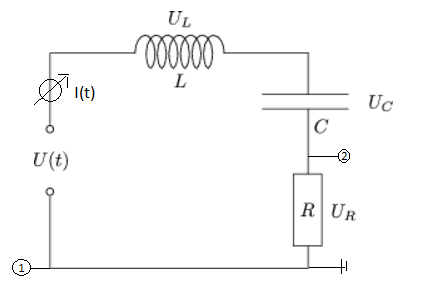
\includegraphics[trim = 0mm 0mm 0mm 0mm,clip, width=9cm]{Bilder/k.png}%
	\caption[Schaltskizze Serienschwingkreis]{Schaltskizze Serienschwingkreis}%
	\label{pic:Abbildung 1}%
\end{figure}
\subsection{Versuchsziel}
Im Folgenden soll der LCR-Serienschwingkreis über seine Güte charakterisiert werden. Dazu werden vier verschiedene Methoden verwendet und die Ergebnisse, sowie deren Genauigkeit verglichen.

\subsection{Herleitung benötigter Formeln}
Aus der Maschenregel folgt für den gezeigten Aufbau die folgende Differentialgleichung:
\begin{eqnarray}
U(t) = U_C(t) + U_L(t) + U_R(t) \\
\Leftrightarrow \frac{U(t)}{L} = \frac{d^2Q}{dt^2} + \frac{R}{L} \cdot \frac{dQ}{dt} + \frac{Q}{L C} \\
\Rightarrow	\frac{1}{L} \cdot \frac{dU}{dt} = \frac{d^2I}{dt^2} + \frac{R}{L} \cdot\frac{I}{t} + \frac{I}{LC}
\end{eqnarray}

Die hier interessante partikuläre Teil der Lösung lässt sich über den Ansatz $U(t) = U_0 \cdot e^{i \omega t} \; und \; I(t) = I_0 \cdot e^{i( \omega t - \phi)}$ bestimmen.\\
Nach Einsetzen in die Differentialgleichung und Aufteilen in Imaginär - und Realteil findet man, dass für die Phase und den Stromamplitude gilt:
\begin{eqnarray}
tan(\phi) = \frac{\omega L - \frac{1}{\omega C}}{R} \\
I_0 = \frac{U_0}{\sqrt{R^2 + (\omega L - \frac{1}{\omega C})^2}} = \frac{U_0}{Z} \\
\Rightarrow Z = \sqrt{R^2 + (\omega L - \frac{1}{\omega C})^2}
\end{eqnarray}
mit Gesamtimpedanz Z. \\
Der Resonanzfall tritt auf für die Resonanzfrequenz $\omega_0 = fraq{1}{\sqrt{L \cdot C}}$, da dort die Impedanz minimal und damit der Strom maximal wird.

\subsubsection{Bestimmung der Güte}
1) Die Güte lässt sichexperimentell aus der Resonanzfrequenz $f_0$ und der Breite $\Delta f$ der Resonanzkurve bzw. aus den äquivalenten Kreisfrequenzen bestimmen. Die Breite der Resonanzkurve ist dabei über die Stellen definiert, an denen die Stromstärke auf den Faktor $\frac{1}{\sqrt{2}}$ des Maximums abfällt.\\
Rechnerisch ergibt sich 
\begin{eqnarray}
\omega_0 = \frac{1}{\sqrt{L \cdot C}} \; und \; \Delta \omega = \frac{R}{L} \\
\Rightarrow Q_1 = \frac{\omega_0}{\Delta \omega}
\end{eqnarray} 

2) Analog kann man die Güte natürlich auch direkt aus den bekannten Kenngrößen der Impedanzen bestimmen:
\begin{equation}
Q_2 = \frac{\omega_0}{\Delta \omega} = \frac{1}{R} \cdot \sqrt{\frac{L}{C}}
\end{equation}

3) Aus der Aufzeichnung der Phasenverschiebung in Abhängigkeit von der Frequenz lassen sich ebenfalls $f_0$ und $\Delta f$ bestimmen. Bei der Resonanzfrequenz verschwindet nämlich die Phasenverschiebung und an den Stellen $f_0 \pm \Delta f$ nimmt die Phasenverschiebung die Werte $\pm 45 \deg$ an. Dann ergibt sich analog zu vorher 
\begin{equation}
Q_3 = \frac{f_0}{\Delta f}
\end{equation}

4) Als letzte Möglichkeit kann man die Güte aus der Spannungsüberhöhung an der Spule errechnen. Es gilt nämlich bei der Resonanzfrequenz 
\begin{equation}
\frac{U_L(\omega_0}{U(\omega_0)} = \frac{I_0 \omega L}{I_0 R} = \frac{1}{R} \cdot \sqrt{\frac{L}{C}} = Q \\
U_L(\omega_0) = I_0 \omega_0 L = I_0 \frac{L}{\sqrt{LC}} = I_0 \frac{1}{\omega_0 C} = U_C(\omega_0)
\end{equation}
Demnach lässt sich die Güte bestimmen, indem man die minimale Spannung $U_1$ und die Spannung des Schnittpunktes $U_2$ von $U_L$ und $U_C$ bestimmt. Dann ergibt sich für die Güte 
\begin{equation}
Q_4 = \frac{U_2}{U_1}
\end{equation}

\subsection{Messung mit dem Oszilloskop}

\subsubsection{Versuchsaufbau}
Für den Versuch werden Kondensator, Spule und Widerstand wie auf der Schaltskizze erkennbar auf die Rastersteckplatte in Serie geschaltet. Als Spannungsquelle dient hier ein Function Generator mit regelbarer Frequenz.
Zusätzlich wird ein Oszilloskop so dazugeschaltet, dass die Masse zwischen Widerstand und dem Function Generator liegt. Channel 1 und 2 werden dann so angeschlossen, dass sich die Gesamtspannung und die am Widerstand abfallende Spannung, welche sich nur um einen Faktor R vom Strom unterscheidet, messen lassen (siehe Schaltskizze).
Die dabei verwendeten Bauteile waren:

\hskip-3.8cm
\renewcommand{\arraystretch}{1.5}
\begin{tabular}{|c|c|c|}
\hline 	$ $ 	&	Gruppe 1	&	Gruppe 2 \\
\hline 	Widerstand 	&	$ R_R = (19.79 \pm 0.05) \Omega$					&	$ (19.83 \pm 0.05) \Omega$	\\
\hline 	Spule		&	$ L = (1.301 \pm 0.004) mH \; (250 \,Windungen) $	&	$ L = (4.776 \pm 0.012) mH \; (500 \,Windungen) $ \\
\hline	Spuleninnenwiderstand	&	$ R_L = (0.745 \pm 0.002) \Omega $	&	$ R_L = (3.855 \pm 0.010) \Omega $ \\
\hline  Gesamtwiderstand	&	$ R = (20.54 \pm 0.05) \Omega$				&	$ R = (23.69 \pm 0.05) \Omega $ \\
\hline 	Kondensator &	$ C = (4.735 \pm 0.012) \mu F$					&	$ C = (4.719 \pm 0.012) \mu F$ \\
\hline	
\end{tabular}
\newline
Hierbei wurden die Bauteile mit Hilfe der Messbrücke ausgemessen. Die Unsicherheit ist dabei vom Hersteller als ein viertel Prozent des Messwertes angegeben.

\subsubsection{Versuchsdurchführung und -Auswertung}
Mit dem Oszilloskop sollte die Güte über die Spannungsüberhöhung bestimmt werden. \\
Zunächst wurden auf dem Oszilloskop $U_R$ und $U$ in der X-Y-Darstellung gegeneinander aufgetragen. Die entstehenden Lissajou-Figuren werden durch Regelung der Frequenz am Function Generator so lange verändert, bis sie eine Gerade bildet. Diese Frequenz ist dann die Resonanzfrequenz, da hier die Phasenverschiebung zwischen Strom und Spannung verschwindet.
Bei der ersten Gruppe wurde eine Frequenz von $f_0 = (2045 \pm \frac{4}{\sqrt{12}}) Hz$ gemessen. Die Unsicherheit ergab sich dabei daraus, dass die Figur für eine Frequenz von $f = 2043 Hz$ oder $f = 2047 Hz$ bereits erkennbar von einer Geraden abwich und dann für den Messwert eine Gleichverteilung in diesem Intervall angenommen wurde.
Zur Bestimmung der Breite wurde dann in die X-t-Darstellung des Oszilloskops gewechselt. Zunächst wurde die Spannungsdifferenz zwischen den Minima und Maxima bestimmt. Der untere Cursor wurde dann nach oben verschoben, so dass sich diese Differenz halbiert und dann wurde noch der obere Cursor nach unten verschoben, so dass die Differenz um einen Faktor $\frac{1}{2\sqrt{2}}$ kleiner ist also zuvor. Hier wurde nun die Frequenz am Function Generator angepasst, so dass die Maxima wieder auf der Cursorlinie lagen. Aus den entsprechenden Frequenzen lässt sich dann die Breite der Resonanzkurve bestimmen.\\
Bei der ersten Gruppe wurden die Frequenzen zu $f_+ = (3700 \pm \frac{40}{\sqrt{12}}) Hz$ und $f_- = (1120 \pm \frac{20}{\sqrt{12}}) Hz$. Auch hier wurde wieder eine Gleichverteilung in den entsprechenden Intervallen angenommen, wobei die Intervallgrenzen dadurch bestimmt wurden, so dass die Maxima erkennbar vom geforderten Wert abwichen.\\
Die selben Messverfahren wurden auch von der zweiten Gruppe angewandt, die Ergebnisse sind in der folgenden Tabelle zusammengefasst:
\begin{center}
\renewcommand{\arraystretch}{1.5}
\begin{tabular}{|c|c|c|}
\hline $ $ 			&	Gruppe 1	&	Gruppe 2 \\
\hline $f_+$ 		&	$ (3700 \pm \frac{40}{\sqrt{12}}) Hz $		&	$(1579 \pm \frac{1}{\sqrt{12}}) Hz$	\\
\hline $f_-$		&	$ (1120 \pm \frac{20}{\sqrt{12}}) Hz $		&	$(726 \pm \frac{1}{\sqrt{12}}) Hz$ \\
\hline $\Delta f$ 	&	$ (2580 \pm 13) Hz$				&	$ (853 \pm 0.3) Hz$ \\
\hline $f_0$		&	$ (2045 \pm \frac{4}{\sqrt{12}}) Hz$	&	$ (1067 \pm \frac{1}{\sqrt{12}}) Hz$ \\
\hline $Q_{exp} = \frac{f_0}{\Delta f}$						&	$ 0.793 \pm 0.004 $	&	$ 1.251 \pm 0.0012$ \\
\hline $Q_{theo} = \frac{1}{R} \cdot \sqrt{\frac{L}{C}}$	&	$ 0.807 \pm 0.003$	&	$ 1.343 \pm 0.005$ \\
\hline Abweichung $\frac{|Q_{exp} - Q_{theo}|}{\sqrt{\sigma_{Q_{exp}}^2 + \sigma_{Q_{theo}}^2}}$ & $ 2.8 $ & $ 17.9 $ \\
\hline
\end{tabular}
\end{center}

Die Unsicherheiten ergeben sich dabei nach Gaußscher Fehlerfortpflanzung zu 
\begin{eqnarray*}
\sigma_{\Delta f} = \sqrt{\sigma_{f_+}^2 + \sigma_{f_-}^2} \\
\sigma_{Q_{exp}} = Q_{exp} \cdot \sqrt{\frac{\sigma_{f_0}^2}{f_0^2} + \frac{\sigma_{\Delta f}^2}{\Delta f^2}} \\
\sigma_{Q_{theo}} = Q_{theo} \cdot \sqrt{\frac{\sigma_R^2}{R^2} + \frac{\sigma_L^2}{4L^2} + \frac{\sigma_C^2}{4C^2}}
\end{eqnarray*}



\subsection{Messung mit dem Sensor-Cassy}
\subsubsection{Versuchsaufbau}
Für den Versuch werden Kondensator, Spule und Widerstand wie auf der Schaltskizze erkennbar auf die Rastersteckplatte in Serie geschaltet. Die Spannungsmessgeräte des Sensor-Cassy werden zudem parallel zum Kondensator bzw. zur Spule geschaltet, um die Spannung, die an diesen Bauteilen abfällt zu messen. \\
Dabei wurden die folgenden Bauteile verwendet:

\hskip-3.8cm
\renewcommand{\arraystretch}{1.5}
\begin{tabular}{|c|c|c|}
\hline 	$ $ 	&	Gruppe 1	&	Gruppe 2 \\
\hline 	Ohmsche Widerstände 	&	$ R_1 = (0.983 \pm 0.003) \Omega$					&	$ R_1 = (5.184 \pm 0.013) \Omega$	\\
\hline 	$ $ 	&	$ R_2 = (5.110 \pm 0.013) \Omega$					&	$ R_2 = (9.955 \pm 0.025) \Omega$	\\
\hline 	$ $ 	&	$ R_3 = (19.79 \pm 0.05) \Omega$					&	$ R_3 = (19.83 \pm 0.05) \Omega$	\\
\hline 	Spule		&	$ L = (1.301 \pm 0.004) mH \; (250 \,Windungen) $	&	$ L = (4.776 \pm 0.012) mH \; (500 \,Windungen) $ \\
\hline	Spuleninnenwiderstand	&	$ R_L = (0.745 \pm 0.002) \Omega $	&	$ R_L = (3.855 \pm 0.010) \Omega $ \\
\hline  Gesamtwiderstände	&	$ R_1 = (1.728 \pm 0.004) \Omega$				&	$ R_5 = (9.039 \pm 0.017) \Omega $ \\
\hline  $ $	&	$ R_5 = (5.855 \pm 0.013 \Omega$				&	$ R_{10} = (13.81 \pm 0.027) \Omega $ \\
\hline  $ $	&	$ R_{20} = (20.54 \pm 0.05) \Omega$				&	$ R_{20} = (23.69 \pm 0.05) \Omega $ \\
\hline 	Kondensator &	$ C = (4.735 \pm 0.012) \mu F$					&	$ C = (4.719 \pm 0.012) \mu F$ \\
\hline	
\end{tabular}
\newline
\newline
Die Unsicherheiten auf die Messwerte werden dabei vom Hersteller der Messbrücke auf ein viertel Prozent des Messwertes angegeben. Für den Gesamtwiderstand errechnet sich die Unsicherheit dann aus der quadratischen Addition der Einzelfehler.

\subsubsection{Versuchsdurchführung}
Für die Messungen wurde zunächst mit dem Power-Cassy eine Sinus-förmige Spannung erzeugt. Die Abfälle der Spannungen an Kondensator und Spule wurden dann mit Hilfe des Sensor-Cassy und der fließende Strom durch das Amperemeter des Power-Cassy als Effektivwerte gemessen.\\
Die dazu zu wählenden Messparameter waren eine Messzeit von 100 ms und eine Messpunktanzahl von 0. \\
Die gemessenen Spannungen uns Ströme werden in Abhängigkeit zur angelegten Frequenz aufgetragen, die während der Messung stückweise in 20 Hertz Schritten erhöht wurde. Um sicherzustellen, dass sich das System bei Aufnahme des Messpunktes nicht mehr im Einschwingvorgang befand, wurde der erst nach einer Wartezeit von 2 Sekunden aufgenommen.\\
Zusätzlich wurde noch die Phasenverschiebung zwischen dem Gesamtstrom und der angelegten Spannung gemessen und ebenfalls in Abhängigkeit von der Frequenz aufgetragen.\\
Die Messung wurde dann mit jedem der angegebenen Widerstände durchgeführt.

\subsection{Versuchsauswertung}
Wie zuvor erläutert, lässt sich die Güte auf verschiedene Arten bestimmen. \\
Zunächst lässt sich aus dem Verlauf der Stromresonanzkurve das Maximum $I_{max}$, sowie die entsprechende Resonanzfrequenz $f_0$ bestimmen.
\begin{center}
\renewcommand{\arraystretch}{1.5}
\begin{tabular}{|c|c|c|c|c|}
\hline verwendeter Widerstand	& $f_{0_1}$	[Hz]&	$f_{0_2}$	[Hz] & $I_{max_1}$ [A]& $I_{max_2}$ [A]\\
\hline $  1 \Omega $		&	$ \pm $	&	$ \pm $	&	$ \pm $	&	$ \pm $ 	\\
\hline $  5 \Omega $		&	$ \pm $	&	$ \pm $	&	$ \pm $	&	$ \pm $ 	\\
\hline $ 10 \Omega $		&	$ \pm $	&	$ \pm $	&	$ \pm $	&	$ \pm $		\\
\hline $ 20 \Omega $		&	$ \pm $	&	$ \pm $	&	$ \pm $	&	$ \pm $		\\
\hline
\end{tabular}
\end{center}
Die Unsicherheiten 
.............................................................\\
.............................................................\\
.............................................................\\
.............................................................\\

Aus den Stellen, an denen die Stromkurve den Wert $\frac{I_{max}}{\sqrt{2}}$ erreicht($f_+$ und $f_-$), kann man zudem die Breite der Kurve $\Delta f = f_+ - f_-$ berechnen.
\begin{center}
\renewcommand{\arraystretch}{1.5}
\begin{tabular}{|c|c|c|c|}
\hline verwendeter Widerstand	& $f_+$	[Hz]&	$f_-$	[Hz] & $\Delta f $ [Hz] 	\\
\hline $  1 \Omega $ Gruppe 1	&	$ \pm $	&	$ \pm $	&	$ \pm $	 	\\
\hline $ 10 \Omega $ Gruppe 1	&	$ \pm $	&	$ \pm $	&	$ \pm $		\\
\hline $ 20 \Omega $ Gruppe 1	&	$ \pm $	&	$ \pm $	&	$ \pm $		\\
\hline $  5 \Omega $ Gruppe 2 	&	$ \pm $	&	$ \pm $	&	$ \pm $	 	\\
\hline $ 10 \Omega $ Gruppe 2	&	$ \pm $	&	$ \pm $	&	$ \pm $		\\
\hline $ 20 \Omega $ Gruppe 2	&	$ \pm $	&	$ \pm $	&	$ \pm $		\\
\hline
\end{tabular}
\end{center}
Die Unsicherheiten 
.............................................................\\
.............................................................\\
.............................................................\\
.............................................................\\





Zum Vergleich lässt sich aus den Charakteristika der verwendeten Impedanzen eine Vorhersage für die Güte berechnen.
\begin{eqnarray*}
Q_{theo} = \frac{\omega_0}{\Delta \omega} = \frac{1}{R} \cdot \sqrt{\frac{L}{C}} \\
\sigma_{Q_{theo}} = Q_{theo} \cdot \sqrt{\frac{\sigma_R^2}{R^2} + \frac{\sigma_L^2}{4L^2} + \frac{\sigma_C^2}{4C^2}}
\end{eqnarray*}
Die Unsicherheit auf den Wert ergibt sich dabei aus der gaußschen Fehlerfortpflanzung. Damit errechnen sich die theoretischen Werte für die Güte zu:

\begin{center}
\renewcommand{\arraystretch}{1.5}
\begin{tabular}{|c|c|c|}
\hline verwendeter Widerstand	&	Gruppe 1	&	Gruppe 2 \\
\hline $  1 \Omega $		&	$ 9.59 \pm 0.03$	&	$ / $ 	\\
\hline $  5 \Omega $		&	$ 2.83 \pm 0.01$	&	$ 3.52 \pm 0.01$ 	\\
\hline $ 10 \Omega $		&	$ / $	&	$ 2.30 \pm 0.01$ 	\\
\hline $ 20 \Omega $		&	$ 0.807 \pm 0.003$	&	$ 1.343 \pm 0.004$ 	\\
\hline
\end{tabular}
\end{center}





\newpage

\section{Parallelschwingkreis}
\begin{figure}[H]
	\centering
	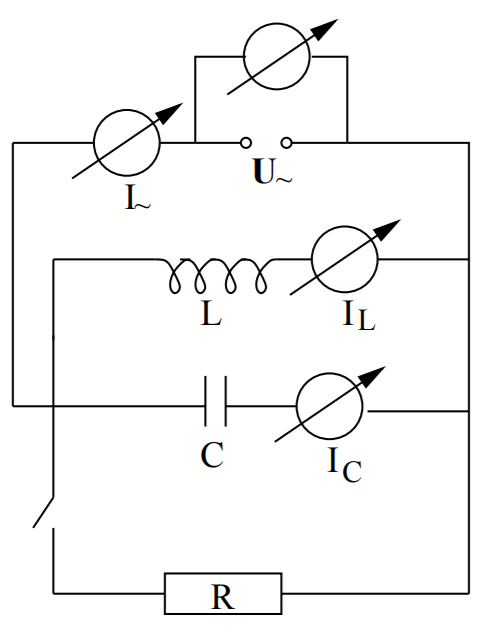
\includegraphics[trim = 0mm 0mm 0mm 0mm,clip, width=6cm]{Bilder/Parallelschwingkreis_Schaltskizze.png}%
	\caption[Schaltskizze Parallelschwingkreis]{Schaltskizze Parallelschwingkreis}%
	\label{pic:Abbildung 2}%
\end{figure}

\subsection{Versuchsziel}
Analog zum Serienschwingkreis soll der LCR-Parallelschwingkreis über seine Güte charakterisiert werden. IM Prinzip werden die selben Methoden verwendet, bloß die Bestimmung der Frequenzen über die Phasenverschiebung ist hier impraktikabel und wird daher nicht durchgeführt.

\subsection{Herleitung benötigter Formeln}
Mit Hilfe der Knotenregel erhält man für die Spannung die Gleichung
\begin{eqnarray*}
I = I_R + I_C + I_L \\
\Leftrightarrow \frac{U}{Z} = \frac{U}{R} + i \omega C \cdot U + \frac{U}{i \omega L + R_L}
\end{eqnarray*}
Damit folgt dann für die Impedanz 
\[ \frac{1}{Z} = \frac{1}{R} + i \omega C + \frac{1}{i \omega L + R_L} = \frac{1}{X_R}  + \frac{1}{X_C} + \frac{1}{X_L} \]
Es werden also die inversen Impedanzen, also die Leitwerte addiert. 
\begin{center}
\renewcommand{\arraystretch}{1.5}
\begin{tabular}{|c|c|}
\hline 	Impedanz 	&	Leitwert \\
\hline 	$X_R = R$ 						&	$Y_R = \frac{1}{R}$	\\
\hline 	$X_C = \frac{1}{i \omega C}$ 	&	$Y_C = i \omega C $	\\
\hline 	$X_L = i \omega L + R_L$ 		&	$Y_L = \frac{R_L}{R}$\\
\hline	
\end{tabular}
\end{center}
Für den Betrag des Gesamtleitwertes $Y$ erhält man daraus 
\[ |Y| = | Y_R + Y_L + Y_C| = \sqrt{ \left(\frac{1}{R} + \frac{R_L}{R_L^2 + \omega^2 L^2} \right)^2 + \left( \omega C - \frac{\omega L}{R_L^2 + \omega^2 L^2} \right)^2} \]
Der Leitwert wird damit minimal, wenn der Imaginärteil verschwindet. Dies ist für die Resonanzfrequenz
\[ \omega_0 = \sqrt{\frac{1-\frac{C}{L} \cdot R_L^2}{LC}} \] erfüllt. An dieser Stelle tritt also Resonanz auf, die Impedanz ist Maximal und damit der Strom minimal.
Aus $ I = Y \cdot U$ erhält man dann mit dem Ansatz $I(t) = I_0 \cdot e^{i(\omega t - \phi)}$ für die Phase und die Stromstärkeamplitude:
\begin{eqnarray}
tan(\phi) = - \frac{\omega C - \frac{\omega L}{R_L^2 + \omega^2 L ^2}}{\frac{1}{R} + \frac{R_L}{R_L^2 + \omega^2 L ^2}} \\
I_0 = |Y| \cdot U_0
\end{eqnarray}

\subsubsection{Messung der Güte}
Drei der vier Methoden zur Bestimmung der Güte des Serienschwingkreises lassen sich in leicht abgewandelter Form auch auf den Parallelschwingkreis anwenden.\\
1) Zunächst kann man die Güte wieder aus der Resonanzfrequenz $f_0$ und der Breite der Resonanzkurve $\Delta f$ bzw. den äquivalenten Kreisfrequenzen bestimmen. Die Breite der Kurve ist dabei durch die Stellen gegeben, an denen der Strom den Wert $\sqrt{2} \cdot I_{min}$ annimmt. \\
Die Güte ergibt sich dann zu \[ Q_1 = \frac{f_0}{\Delta f} \]

2) An der Resonanzstelle gilt ähnlich zum Serienschwingkreis (Ströme statt Spannungen): \[ I_L(\omega_0) = I_C(\omega_0) \] und \[ Q = \frac{I_L(\omega_0)}{I(\omega_0)} \]
Man kann also hier den Schnittpunkt der Stromkurven von Spule und Kondensator bestimmen ($I_2$) und diesen mit dem Stromminimum der Resonanzkurve vergleichen und erhält daraus \[Q_2 = \frac{I_2}{I_{min}} \]

3) Natürlich kann man auch wieder die Güte direkt aus den Charakteristika der Impedanzen errechnen. 
\[ Q_3 = \frac{I_L(\omega_0)}{I(\omega_0)} = \frac{U_0}{\omega_0 L} \cdot \frac{Z(\omega_0)}{U_0} = \frac{R \cdot \sqrt{ \frac{C}{L}}}{1 + R \cdot R_L \cdot \frac{C}{L}} \]


\subsection{Versuchsaufbau}
Bei diesem Teilversuch wurden Spule, Kondensator und Widerstand entsprechend der Schaltskizze angeordnet, also parallel zueinander geschaltet. Da bei einer solchen Anordnung die abfallende Spannung an allen Bauteilen gleich ist, wurden die durch Spule und Kondensator fließenden Ströme gemessen. Das zur Strommessung verwendete Sensor-Cassy muss dazu jeweils zur Spule bzw. zum Kondensator in Reihe geschaltet werden. Als Spannungsquelle diente wieder das Power-Cassy.
In diesem Versuchsteil wurden die folgenden Bauteile verwendet:

\hskip-3.8cm
\renewcommand{\arraystretch}{1.5}
\begin{tabular}{|c|c|c|}
\hline 	$ $ 	&	Gruppe 1	&	Gruppe 2 \\
\hline 	Ohmsche Widerstände 	&	$ R_{R_1} = (0.983 \pm 0.003) \Omega$					&	$ R_{R_1} = (5.184 \pm 0.013) \Omega$	\\
\hline 	$ $ 	&	$ R_{R_2} = (5.110 \pm 0.013) \Omega$					&	$ R_{R_2} = (9.955 \pm 0.025) \Omega$	\\
\hline 	Spule		&	$ L = (1.301 \pm 0.004) mH \; (250 \,Windungen) $	&	$ L = (4.776 \pm 0.012) mH \; (500 \,Windungen) $ \\
\hline	Spuleninnenwiderstand	&	$ R_L = (0.745 \pm 0.002) \Omega $	&	$ R_L = (3.855 \pm 0.010) \Omega $ \\
\hline 	Kondensator &	$ C = (4.735 \pm 0.012) \mu F$					&	$ C = (4.719 \pm 0.012) \mu F$ \\
\hline	
\end{tabular}
\newline
\newline
Die Unsicherheiten auf die Messwerte werden dabei vom Hersteller der Messbrücke auf ein viertel Prozent des Messwertes angegeben.


\subsection{Versuchsdurchführung}
Genau wie beim Serienschwingkreis wurde mit dem Power-Cassy eine Sinus-förmige Spannung erzeugt. Die durch Spule und Kondensator fließenden Ströme wurden mit dem Sensor-Cassy (Eingang A) und der Gesamtstrom mit dem Amperemeter des Power-Cassy als Effektivwerte gemessen.\\
Die dazu zu wählenden Messparameter waren eine Messzeit von 100 ms und eine Messpunktanzahl von 0.\\
Die gemessenen Ströme wurden wieder gegen die Frequenz der angelegten Spannung aufgetragen, die während der Messung stückweise in 20 Hertz Schritten erhöht wurde. Um sicherzustellen, dass sich das System bei Aufnahme des Messpunktes nicht mehr im Einschwingvorgang befand, wurde der erst nach einer Wartezeit von 2 Sekunden aufgenommen.\\
Die Messung wurde zunächst jeweils für die beiden angegebenen Widerstände durchgeführt. Dann wurde der Widerstand aus der Schaltung entfernt (dies entspricht einem unendlichen Widerstand), so dass man einen LC-Parallelschwingkreis erhält, für den die Messung ein weiteres Mal durchgeführt wurde.

\subsection{Versuchsauswertung}



\newpage
\section{Hoch- und Tiefpassfilter}
Als eigenständiger Versuch war es Aufgabe, aus einem Widerstand und einem Kondensator oder einer Spule, einen Frequenzfilter zu erstellen. Bei einem solchen Hoch- oder Tiefpass sind die Bauteile in Reihe geschaltet.
\newline
\begin{figure}[H]
	\hskip -0.5cm
	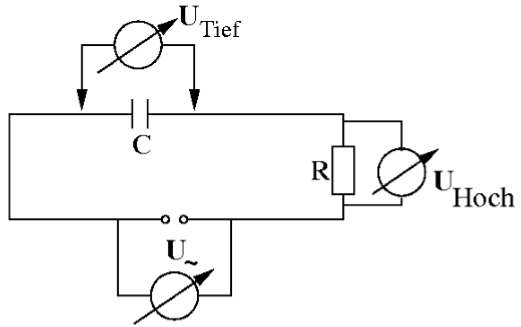
\includegraphics[trim = 0mm 0mm 0mm 0mm,clip, width=11cm]{Bilder/Schaltskizze_Filter.png}%
	\caption[Schaltskizze Hoch- bzw Tiefpass]{Schaltskizze Hoch- bzw Tiefpass}%
	\label{pic:Abbildung 1}%
\end{figure}
Wie hier zu erkennen, hängt es nur davon ab wo die Spannung mit Cassy gemessen wird, ob der Filter als Hoch- oder Tiefpass fungiert. Die Übertragungsfunktion ergibt sich als Quotient der Ausgangsspannung und der Eingangsspannung zu:
\newline
\newline
Hochpass: $\frac{U_a}{U_e}=\frac{1}{\sqrt{(\frac{1}{\omega \cdot C \cdot R})^2+1}}$ 
\newline
Tiefpass: \, $\frac{U_a}{U_e}=\frac{1}{\sqrt{1+(\omega \cdot R \cdot C)^2}}$
\newline
\newline
Offensichtlich gilt in den Grenzfällen: 
\newline
\newline
$\lim\limits_{R \rightarrow \infty}{\frac{U_a}{U_e}}$:\;\;\; $(\frac{U_a}{U_e})_{Hoch} \rightarrow  1$ und $(\frac{U_a}{U_e})_{Tief} \rightarrow 0$
\newline und
\newline
 $\lim\limits_{R  \to 0}{\frac{U_a}{U_e}}$:  \;\;\; $(\frac{U_a}{U_e})_{Hoch} \rightarrow  0$ und $(\frac{U_a}{U_e})_{Tief} \rightarrow 1$
\newline
\begin{figure}[H]
	\hskip -2cm
	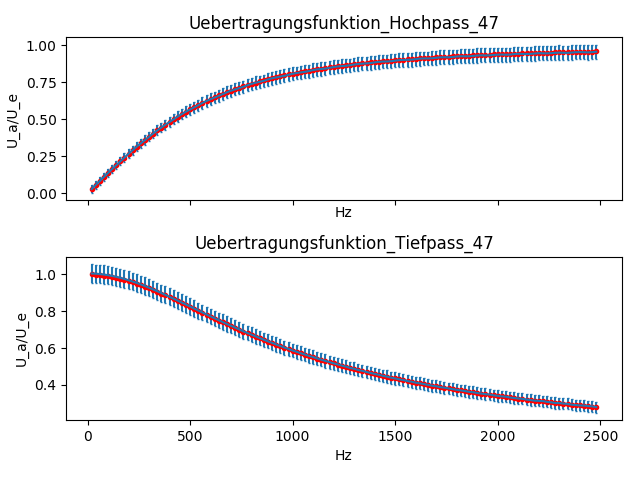
\includegraphics[trim = 0mm 0mm 0mm 0mm,clip, width=17cm]{Bilder/Uebertragungsfunktionen47.png}%
	\caption[Übertragungsfunktionen Gruppe 2 (vertikale Striche nur zur besseren Übersicht, keine Fehlerbalken)]{Übertragungsfunktionen Gruppe 2 (vertikale Striche nur zur besseren Übersicht, keine Fehlerbalken)}%
	\label{pic:Abbildung 1}%
\end{figure}
An diesem Graphen der Übertragungsfunktion lässt sich erkennen, das die gemessenen Werte (blau) sehr eng an den theoretischen (rot) liegen. Das sich das asymptotische Verhalten gegen 1 bzw gegen 0, hier nicht bzw schlecht erkennen lässt, ist eine Folge des zu kurz gewählten Messbereichs der endet bevor asymptotisches Verhalten vorlag.
\newline
\newline
In der Regel werden solche Filter über ihre Grenzfrequenz charakterisiert. Die Grenzfrequenz, $\omega_0$, erfüllt die Bedingung $\frac{U_a}{U_e}(\omega_0)=\frac{1}{\sqrt{2}}$. Demnach gilt hier $\omega_0=\frac{1}{R \cdot C}$.
Dadurch ergibt sich aufgrund der Theorie:
\newline
\begin{center}
\renewcommand{\arraystretch}{1.5}
\begin{tabular}{|c|c|c|c|}
\hline 	$ $ & Widerstand 	&	Kondensator	&	Grenzfrequenz  \\
\hline 	Gruppe 1 	&	$ R = (46.69 \pm 0.12) \Omega $ & $ C = (4.735 \pm 0.012) \mu F $ & $ f_0 = (719.91 \pm 2.60) Hz$	\\
\hline 	Gruppe 2		&	$ R=(46.55 \pm 0.12) \Omega $	&	$C = (4.719 \pm 0.012) \mu F $ &$ f_0 = (724.52 \pm 1.82) Hz$ \\
\hline 	Gruppe 2 &	$ R=(19.83 \pm 0.05) \Omega $					&	$C = (4.719 \pm 0.012) \mu F $ & $ f_0 = (1700.78 \pm 4.52) Hz$ \\
\hline	
\end{tabular}
\end{center}
\newpage
Aus den Messwerten lässt sich bestimmen:
\newline
\begin{center}
\renewcommand{\arraystretch}{1.5}
\begin{tabular}{|c|c|c|c|c|}
\hline 	$ Messung $ & $f_{Hochpass}$& $f_{Tiefpass}$	&	$Abweichung_{H}( in\; \sigma)$ & $Abweichung_{T}( in\; \sigma)$  \\
\hline 	Gruppe 1 	&	$(740 \pm 12) Hz$& $(700 \pm 12)Hz$ &$ 1.70$& $1.68$	\\
\hline 	Gruppe 2		&	 $(720 \pm 12) Hz$ 	&	$(720 \pm 12) Hz $ &$ 0.39 $&$0.39 $ \\
\hline 	Gruppe 2 &	 $(1740 \pm 12) Hz$ 					&	$(1700 \pm 12) Hz $ & $3.18$ & $0.06$ \\
\hline	
\end{tabular}
\end{center}
Die Unsicherheiten auf die charakteristischen Größen der Bauteile sind hier systematischer Natur und durch den Hersteller als $0,0025\%$ des gemessenen Wertes gegeben. Denn der systematische Unsicherheit liegt hier über dem statistischen Unsicherheit der Ablesegenauigkeit, und macht somit den größeren Teil aus. Durch Fehlerfortpflanzung ergeben sich so die Fehler auf den theoretischen Wert von $f_0$ zu:
\newline
$\sigma_{f_{0_{theo}}}=\sqrt{(\frac{1}{R^2 \cdot C})^2 \cdot \sigma_{R}^2+(\frac{1}{R \cdot C^2})^2 \cdot \sigma_{C}^2}$
\newline
Die Unsicherheiten auf die gemessenen Grenzfrequenzen ergibt sich zum einen aus der Schrittweite in der das Frequenzspektrum durchlaufen wurde, das waren hier 20 Hz nimmt man eine Gleichverteilung an gibt das einen Ablesefehler von $\sigma_{ablese}=\frac{20}{\sqrt{3}}$. Da die Spannungsmessung durch Sensor-Cassy vom Hersteller aus mit der Unsicherheit $\sigma_U=0.01 \cdot U_i+0.005 \cdot U_{Bereichsendwert}$ ergibt sich für die Übertragungsfunktion $f=\frac{U_a}{U_e}$ der Fehler $\sigma_f^2=(\frac{1}{U_e})^2 \cdot \sigma_{U_a}^2+(\frac{U_a}{U_e^2})^2+\sigma_{U_e}^2$
Damit ist die Unsicherheit auf die Grenzfrequenz $\sigma_{f_0}=\sqrt{\sigma_f^2+\sigma_{ablese}^2}$
\newline
Die Abweichung zwischen Theorie und Messwert ist als $\delta=\frac{|f_{theo}-f_{mess}|}{\sqrt{(\sigma_{f_0})^2+(\sigma_{f_{0_{theo}}})^2}}$ zu berechnen.
\newline
Bei Betrachtung beider Tabellen fällt sofort auf das die Grenzfrequenz für Hoch- und Tiefpass, nur in einem von drei Fällen übereinstimmen. Dies sollte jedoch nach Theorie immer der Fall sein. Weiter fällt auf das bei der zweiten Variante von Gruppe 2 die Abweichung stark schwanken, sodass davon auszugehen ist das Messfehler beim Hochpass unterschätzt wurden.
\end{document}